% questions.tex —— 2017 年·全国Ⅲ卷·文科 · 题目内容片段（无答案）
% 由 tools/generate_projects.py 依来源总账自 2017/2017_数学真题_全国3文_试题.md 生成，勿手改（改源 MD 后重跑）


\gkpart{数学}

\begin{gktip}
\textbf{来源说明}：本题面依据固定源 PDF 两页 A3 页面逐题核对，原卷印刷页码 1047–1048。固定源不附答案；本文件仅为题面规范源。
\end{gktip}

\gkpart{一、选择题}

\begin{question}
\gkti{1}已知集合 \(A=\{1,2,3,4\}\)，\(B=\{2,4,6,8\}\)，则 \(A\cap B\) 中元素的个数为（　）。

（A）1　　（B）2　　（C）3　　（D）4

\end{question}
\begin{question}
\gkti{2}复平面内表示复数 \(z=i(-2+i)\) 的点位于（　）。

（A）第一象限　　（B）第二象限　　（C）第三象限　　（D）第四象限

\Needspace{0.4\textheight}
\end{question}
\begin{question}
\gkti{3}某城市为了了解游客人数的变化规律，提高旅游服务质量，收集并整理了 2014 年 1 月至 2016 年 12 月期间月接待游客量（单位：万人）的数据，绘制了下面的折线图。
\nopagebreak[4]
\begin{center}\begin{tikzpicture}[x=0.28cm,y=0.25cm,line cap=round,line join=round,font=\scriptsize]
\draw[->] (0,0)--(37,0);
\draw[->] (0,0)--(0,21);
\foreach \y/\lab in {0/25,5/30,10/35,15/40,20/45} {
  \draw[densely dashed,gray!65] (0,\y)--(36.5,\y);
  \node[left] at (0,\y) {\lab};
}
\foreach \x in {1,...,36} {
  \draw (\x,0)--(\x,-0.35);
  \pgfmathtruncatemacro{\month}{mod(\x-1,12)+1}
  \node[below] at (\x,-0.55) {\month};
}
\draw[thick] plot[mark=*,mark size=0.65pt] coordinates {
  (1,1.5)(2,2.5)(3,2)(4,4)(5,3.5)(6,3)(7,8)(8,10)(9,5.5)(10,7)(11,4.5)(12,3.5)
  (13,6)(14,6.5)(15,5.5)(16,7)(17,7)(18,6)(19,11)(20,12.5)(21,8.5)(22,10)(23,7.5)(24,7)
  (25,7.5)(26,8)(27,10)(28,11.5)(29,11)(30,10)(31,9)(32,14.5)(33,17)(34,12)(35,14)(36,10)
};
\draw (0.1,-0.15)--(-0.1,0.05)--(0.1,0.25);
\node[left] at (-0.25,-0.85) {$O$};
\node at (18,22.4) {月接待游客量（万人）};
\node at (6.5,-2.2) {2014 年};
\node at (18.5,-2.2) {2015 年};
\node at (30.5,-2.2) {2016 年};
\end{tikzpicture}
\end{center}
\nopagebreak[4]
根据该折线图，下列结论错误的是（　）。

（A）月接待游客量逐月增加
（B）年接待游客量逐年增加
（C）各年的月接待游客量高峰期大致在 7、8 月
（D）各年 1 月至 6 月的月接待游客量相对于 7 月至 12 月，波动性更小，变化比较平稳

\end{question}
\begin{question}
\gkti{4}已知 \(\sin\alpha-\cos\alpha=\dfrac{4}{3}\)，则 \(\sin 2\alpha=\)（　）。

（A）\(-\dfrac{7}{9}\)　　（B）\(-\dfrac{2}{9}\)　　（C）\(\dfrac{2}{9}\)　　（D）\(\dfrac{7}{9}\)

\end{question}
\begin{question}
\gkti{5}设 \(x,y\) 满足约束条件
\nopagebreak[4]
\[
\begin{cases}
3x+2y-6\leq 0,\\
x\geq 0,\\
y\geq 0,
\end{cases}
\]
则 \(z=x-y\) 的取值范围是（　）。

（A）\([-3,0]\)　　（B）\([-3,2]\)　　（C）\([0,2]\)　　（D）\([0,3]\)

\end{question}
\begin{question}
\gkti{6}函数
\nopagebreak[4]
\[
f(x)=\frac{1}{5}\sin\left(x+\frac{\pi}{3}\right)+\cos\left(x-\frac{\pi}{6}\right)
\]
的最大值为（　）。

（A）\(\dfrac{6}{5}\)　　（B）1　　（C）\(\dfrac{3}{5}\)　　（D）\(\dfrac{1}{5}\)

\Needspace{0.4\textheight}
\end{question}
\begin{question}
\gkti{7}函数
\nopagebreak[4]
\[
y=1+x+\frac{\sin x}{x^2}
\]
的部分图象大致为（　）。
\nopagebreak[4]
\begin{center}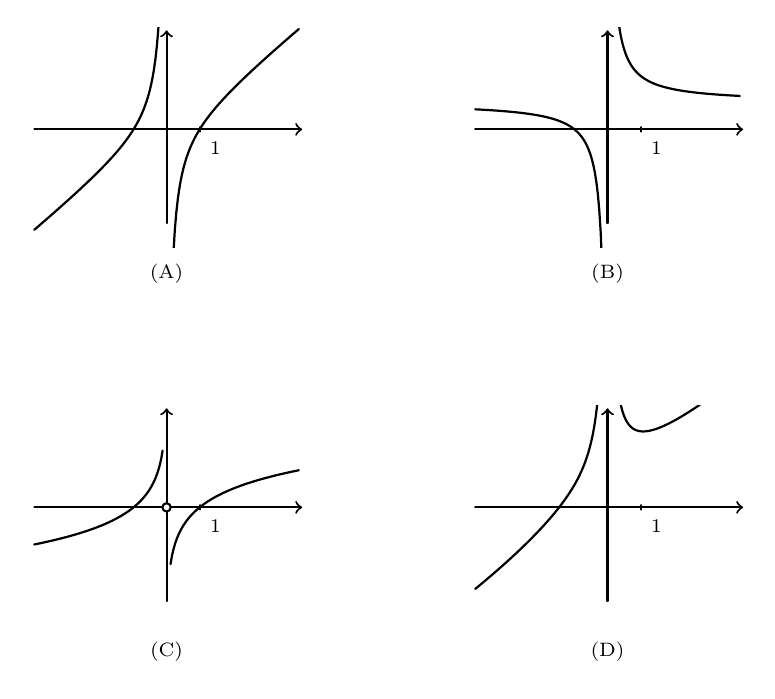
\begin{tikzpicture}[line cap=round,line join=round,line width=0.75pt,font=\scriptsize]
\begin{scope}[shift={(0,4.8)},x=0.42cm,y=0.34cm]
  \begin{scope}
  \clip (-4.2,-4.4) rectangle (4.2,3.8);
  \draw[->] (-4,0)--(4.1,0) node[right] {$x$};
  \draw[->] (0,-3.5)--(0,3.7) node[above] {$y$};
  \draw (1,0.08)--(1,-0.08) node[below right] {$1$};
  \draw[thick,domain=-4:-0.12,samples=90] plot (\x,{\x-1/\x});
  \draw[thick,domain=0.12:4,samples=90] plot (\x,{\x-1/\x});
  \end{scope}
  \node at (0,-5.4) {(A)};
\end{scope}
\begin{scope}[shift={(5.6,4.8)},x=0.42cm,y=0.34cm]
  \begin{scope}
  \clip (-4.2,-4.4) rectangle (4.2,3.8);
  \draw[->] (-4,0)--(4.1,0) node[right] {$x$};
  \draw[->] (0,-3.5)--(0,3.7) node[above] {$y$};
  \draw (1,0.08)--(1,-0.08) node[below right] {$1$};
  \draw[thick,domain=-4:-0.12,samples=90] plot (\x,{1+1/\x});
  \draw[thick,domain=0.12:4,samples=90] plot (\x,{1+1/\x});
  \end{scope}
  \node at (0,-5.4) {(B)};
\end{scope}
\begin{scope}[shift={(0,0)},x=0.42cm,y=0.34cm]
  \begin{scope}
  \clip (-4.2,-4.4) rectangle (4.2,3.8);
  \draw[->] (-4,0)--(4.1,0) node[right] {$x$};
  \draw[->] (0,-3.5)--(0,3.7) node[above] {$y$};
  \draw (1,0.08)--(1,-0.08) node[below right] {$1$};
  \draw[thick,domain=-4:-0.12,samples=90] plot (\x,{-ln(-\x)});
  \draw[thick,domain=0.12:4,samples=90] plot (\x,{ln(\x)});
  \filldraw[fill=white] (0,0) circle (1.5pt);
  \end{scope}
  \node at (0,-5.4) {(C)};
\end{scope}
\begin{scope}[shift={(5.6,0)},x=0.42cm,y=0.34cm]
  \begin{scope}
  \clip (-4.2,-4.4) rectangle (4.2,3.8);
  \draw[->] (-4,0)--(4.1,0) node[right] {$x$};
  \draw[->] (0,-3.5)--(0,3.7) node[above] {$y$};
  \draw (1,0.08)--(1,-0.08) node[below right] {$1$};
  \draw[thick,domain=-4:-0.12,samples=120] plot (\x,{1+\x+sin(deg(\x))/(\x^2)});
  \draw[thick,domain=0.12:4,samples=120] plot (\x,{1+\x+sin(deg(\x))/(\x^2)});
  \end{scope}
  \node at (0,-5.4) {(D)};
\end{scope}
\end{tikzpicture}
\end{center}
\nopagebreak[4]
\Needspace{0.4\textheight}
\end{question}
\begin{question}
\gkti{8}执行如图的程序框图，为使输出 \(S\) 的值小于 91，则输入的正整数 \(N\) 的最小值为（　）。
\nopagebreak[4]
\begin{center}\begin{tikzpicture}[line width=0.75pt,line cap=round,line join=round,font=\small]
\node[draw,rounded corners,minimum width=1.35cm,minimum height=0.5cm] (start) at (0,0) {开始};
\node[draw,minimum width=2.1cm,minimum height=0.55cm] (input) at (0,-0.95) {输入 $N$};
\node[draw,minimum width=3.7cm,minimum height=0.55cm] (init) at (0,-1.9) {$t=1,\ M=100,\ S=0$};
\coordinate (dt) at (0,-2.6);
\coordinate (dr) at (1.7,-3.15);
\coordinate (db) at (0,-3.7);
\coordinate (dl) at (-1.7,-3.15);
\draw (dt)--(dr)--(db)--(dl)--cycle;
\node at (0,-3.15) {$t\le N$};
\node[draw,minimum width=2.8cm,minimum height=0.55cm] (sum) at (0,-4.45) {$S=S+M$};
\node[draw,minimum width=2.6cm,minimum height=0.55cm] (decay) at (0,-5.35) {$M=-M/10$};
\node[draw,minimum width=2.6cm,minimum height=0.55cm] (next) at (0,-6.25) {$t=t+1$};
\node[draw,minimum width=1.9cm,minimum height=0.55cm] (out) at (3.5,-3.15) {输出 $S$};
\node[draw,rounded corners,minimum width=1.35cm,minimum height=0.5cm] (end) at (3.5,-4.15) {结束};
\draw[->] (start)--(input);
\draw[->] (input)--(init);
\draw[->] (init)--(dt);
\draw[->] (db)--node[right]{是}(sum);
\draw[->] (sum)--(decay);
\draw[->] (decay)--(next);
\draw[->] (next.west)--(-2.4,-6.25)--(-2.4,-3.15)--(dl);
\draw[->] (dr)--node[above]{否}(out.west);
\draw[->] (out)--(end);
\end{tikzpicture}
\end{center}
\nopagebreak[4]
（A）5　　（B）4　　（C）3　　（D）2

\end{question}
\begin{question}
\gkti{9}已知圆柱的高为 1，它的两个底面的圆周在直径为 2 的同一个球的球面上，则该圆柱的体积为（　）。

（A）\(\pi\)　　（B）\(\dfrac{3\pi}{4}\)　　（C）\(\dfrac{\pi}{2}\)　　（D）\(\dfrac{\pi}{4}\)

\end{question}
\begin{question}
\gkti{10}在正方体 \(ABCD-A_1B_1C_1D_1\) 中，\(E\) 为棱 \(CD\) 的中点，则（　）。

（A）\(A_1E\perp DC_1\)　　（B）\(A_1E\perp BD\)　　（C）\(A_1E\perp BC_1\)　　（D）\(A_1E\perp AC\)

\end{question}
\begin{question}
\gkti{11}已知椭圆 \(C:\dfrac{x^2}{a^2}+\dfrac{y^2}{b^2}=1\)（\(a>b>0\)）的左、右顶点分别为 \(A_1,A_2\)，且以线段 \(A_1A_2\) 为直径的圆与直线 \(bx-ay+2ab=0\) 相切，则 \(C\) 的离心率为（　）。

（A）\(\dfrac{\sqrt{6}}{3}\)　　（B）\(\dfrac{\sqrt{3}}{3}\)　　（C）\(\dfrac{\sqrt{2}}{3}\)　　（D）\(\dfrac{1}{3}\)

\end{question}
\begin{question}
\gkti{12}已知函数
\nopagebreak[4]
\[
f(x)=x^2-2x+a\left(e^{x-1}+e^{-x+1}\right)
\]
有唯一零点，则 \(a=\)（　）。

（A）\(-\dfrac{1}{2}\)　　（B）\(\dfrac{1}{3}\)　　（C）\(\dfrac{1}{2}\)　　（D）1

\end{question}
\gkpart{二、填空题}

\begin{question}
\gkti{13}已知向量 \(\vec a=(-2,3)\)，\(\vec b=(3,m)\)，且 \(\vec a\perp\vec b\)，则 \(m=\underline{\qquad}\)。

\end{question}
\begin{question}
\gkti{14}双曲线 \(\dfrac{x^2}{a^2}-\dfrac{y^2}{9}=1\)（\(a>0\)）的一条渐近线方程为 \(y=\dfrac{3}{5}x\)，则 \(a=\underline{\qquad}\)。

\end{question}
\begin{question}
\gkti{15}\(\triangle ABC\) 内角 \(A,B,C\) 的对边分别为 \(a,b,c\)，已知 \(C=60^\circ\)，\(b=\sqrt{6}\)，\(c=3\)，则 \(A=\underline{\qquad}\)。

\end{question}
\begin{question}
\gkti{16}设函数
\nopagebreak[4]
\[
f(x)=
\begin{cases}
x+1,&x\leq 0,\\
2^x,&x>0,
\end{cases}
\]
则满足 \(f(x)+f\left(x-\dfrac{1}{2}\right)>1\) 的 \(x\) 的取值范围是 \(\underline{\qquad}\)。

\end{question}
\gkpart{三、解答题}

\begin{question}
\gkti{17}设数列 \(\{a_n\}\) 满足
\nopagebreak[4]
\[
a_1+3a_2+\cdots +(2n-1)a_n=2n.
\]

（1） 求 \(\{a_n\}\) 的通项公式；
（2） 求数列 \(\left\{\dfrac{a_n}{2n+1}\right\}\) 的前 \(n\) 项和。

\end{question}
\begin{question}
\gkti{18}某超市计划按月订购一种酸奶，每天进货量相同，进货成本每瓶 4 元，售价每瓶 6 元，未售出的酸奶降价处理，以每瓶 2 元的价格当天全部处理完。根据往年销售经验，每天需求量与当天最高气温（单位：\(^\circ\mathrm C\)）有关。如果最高气温不低于 25，需求量为 500 瓶；如果最高气温位于区间 \([20,25)\)，需求量为 300 瓶；如果最高气温低于 20，需求量为 200 瓶。为了确定六月份的订购计划，统计了前三年六月份各天的最高气温数据，得下面的频数分布表：

\begin{center}
\begin{tabular}{lrrrrrr}
\toprule
最高气温 & \([10,15)\) & \([15,20)\) & \([20,25)\) & \([25,30)\) & \([30,35)\) & \([35,40)\) \\
\midrule
天数 & 2 & 16 & 36 & 25 & 7 & 4 \\
\bottomrule
\end{tabular}
\end{center}

以最高气温位于各区间的频率代替最高气温位于该区间的概率。

（1） 估计六月份这种酸奶一天的需求量不超过 300 瓶的概率；
（2） 设六月份一天销售这种酸奶的利润为 \(Y\)（单位：元），当六月份这种酸奶一天的进货量为 450 瓶时，写出 \(Y\) 的所有可能值，并估计 \(Y\) 大于零的概率。

\Needspace{0.4\textheight}
\end{question}
\begin{question}
\gkti{19}如图，四面体 \(ABCD\) 中，\(\triangle ABC\) 是正三角形，\(AD=CD\)。
\nopagebreak[4]
\begin{center}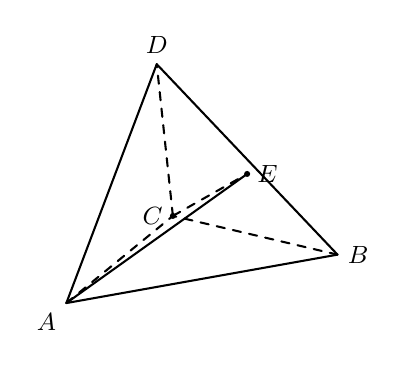
\begin{tikzpicture}[x=0.82cm,y=0.82cm,line cap=round,line join=round,line width=0.75pt,font=\small]
\coordinate (A) at (0,0);
\coordinate (B) at (4.2,0.75);
\coordinate (D) at (1.4,3.7);
\coordinate (C) at (1.65,1.35);
\coordinate (E) at (2.8,2.0);
\draw (A)--(B)--(D)--cycle;
\draw[dashed] (A)--(C)--(B);
\draw[dashed] (C)--(D);
\draw (A)--(E);
\draw[dashed] (C)--(E);
\fill (C) circle (1.1pt);
\fill (E) circle (1.1pt);
\node[below left] at (A) {$A$};
\node[right] at (B) {$B$};
\node[above] at (D) {$D$};
\node[left] at (C) {$C$};
\node[right] at (E) {$E$};
\end{tikzpicture}
\end{center}
\nopagebreak[4]
（1） 证明：\(AC\perp BD\)；
（2） 已知 \(\triangle ACD\) 是直角三角形，\(AB=BD\)，若 \(E\) 为棱 \(BD\) 上与 \(D\) 不重合的点，且 \(AE\perp EC\)，求四面体 \(ABCE\) 与四面体 \(ACDE\) 的体积比。

\end{question}
\begin{question}
\gkti{20}在直角坐标系中 \(xOy\)，曲线 \(y=x^2+mx-2\) 与 \(x\) 轴交于 \(A,B\) 两点，点 \(C\) 的坐标为 \((0,1)\)，当 \(m\) 变化时，解答下列问题：

（1） 能否出现 \(AC\perp BC\) 的情况？说明理由；
（2） 证明过 \(A,B,C\) 三点的圆在 \(y\) 轴上截得的弦长为定值。

\end{question}
\begin{question}
\gkti{21}已知函数
\nopagebreak[4]
\[
f(x)=\ln x+ax^2+(2a+1)x.
\]

（1） 讨论 \(f(x)\) 的单调性；
（2） 当 \(a<0\) 时，证明 \(f(x)\leq-\dfrac{3}{4a}-2\)。

\end{question}
\begin{question}
\gkti{22}在直角坐标系 \(xOy\) 中，直线 \(l_1\) 的参数方程为
\nopagebreak[4]
\[
\begin{cases}
x=2+t,\\
y=kt,
\end{cases}
\quad(t\text{ 为参数}),
\]
\Needspace{5\baselineskip}
直线 \(l_2\) 的参数方程为
\nopagebreak[4]
\[
\begin{cases}
x=-2+m,\\
y=\dfrac{m}{k},
\end{cases}
\quad(m\text{ 为参数}).
\]
设 \(l_1\) 与 \(l_2\) 的交点为 \(P\)，当 \(k\) 变化时，\(P\) 的轨迹为曲线 \(C\)。

（1） 写出 \(C\) 的普通方程；
\Needspace{5\baselineskip}
（2） 以坐标原点为极点，\(x\) 轴正半轴为极轴建立极坐标系，设
\nopagebreak[4]
\[
l_3:\rho(\cos\theta+\sin\theta)-\sqrt{2}=0,
\]
\(M\) 为 \(l_3\) 与 \(C\) 的交点，求 \(M\) 的极径。

\end{question}
\begin{question}
\gkti{23}已知函数 \(f(x)=|x+1|-|x-2|\)。

（1） 求不等式 \(f(x)\geq 1\) 的解集；
（2） 若不等式 \(f(x)\geq x^2-x+m\) 的解集非空，求 \(m\) 的取值范围。

\end{question}